%% abntex2.latex, v<VERSION> dudektria
%% Copyright 2012-2015 by abnTeX2 group at http://abntex2.googlecode.com/ 
%%
%% This work may be distributed and/or modified under the
%% conditions of the LaTeX Project Public License, either version 1.3
%% of this license or (at your option) any later version.
%% The latest version of this license is in
%%   http://www.latex-project.org/lppl.txt
%% and version 1.3 or later is part of all distributions of LaTeX
%% version 2005/12/01 or later.
%%
%% This work has the LPPL maintenance status `maintained'.
%% 
%% The Current Maintainer of this work is Felipe Schneider.
%% Further information are available on http://abntex2.googlecode.com/

%%%%%%%%%%%%%%%%%%%%%%%%%%%%% USO %%%%%%%%%%%%%%%%%%%%%%%%%%%%%%%%%%%%%%%%%%%%%%
%
% Este é um template para o pandoc compatível com abntex2
%
% É necessário chamar pandoc com pelo menos -V documentclass=abntex2 e
% --template=/caminho/absoluto/para/abntex2.latex
%
% Desta maneira, classes baseadas na abntex2 ainda podem ser usadas. O caminho
% absoluto é devido ao fato de o pandoc ter problemas com caminhos relativos.
%
% Todos os exemplos foram compilados com as seguintes opções (exceto quando
% eles mesmos dizem o contrário):
%
%   pandoc -V documentclass=abntex2 \
%          --template=/caminho/absoluto/para/abntex2.latex \
%          -SRs --normalize --filter=pandoc-citeproc \
%          -V lang=english,french,spanish,german,brazil -V papersize=a4paper \
%          -V fontsize=12pt -V classoption=twoside -V classoption=openright \
%          -V linkcolor=blue caminho/do/arquivo.md -o caminho/do/arquivo.pdf
%
% Os com _art.pdf no final receberam também -V classoption=article
% Trocando a extensão do arquivo final de .pdf para .latex gera-se o código
% fonte, para processamento adicional posterior
%
%%%%%%%%%%%%%%%%%%%%%%%%%%%%% METADATA %%%%%%%%%%%%%%%%%%%%%%%%%%%%%%%%%%%%%%%%%
%
% As seguintes metadatas relacionadas ao abntex2 estão disponíveis no template:
% - title:			título do trabalho (caso não haja capa será chamado
%					\maketitle)
% - date:			data
% - author:			autor(es) do trabalho
% - place:			local
% - institution:	instituição
% - preamble:		ver documentação do abntex2 (\preambulo{})
% - abstract:		texto do resumo
% - tags:			lista de palavras-chave (aparece se abstract for definido)
% - tagstitle:		nome para substituir "Palavras-chave" no texto
% - capa:			se true chama \imprimircapa
% - folhaderosto:	se true chama \imprimirfolhaderosto
% - tipotrabalho:	ver documentação do abntex2
%
%%%%%%%%%%%%%%%%%%%%%%%%%%%%% CITAÇÕES %%%%%%%%%%%%%%%%%%%%%%%%%%%%%%%%%%%%%%%%%
%
% São feitas pelo pandoc-citeproc (chame pandoc --filter=pandoc-citeproc).
% Isto quer dizer que você precisa chamar
%
%   \postextual
%   # Referências
%
% ou algo semelhante no final do seu markdown. Para citar use as metadatas
% bibliography e csl como descrito na documentação do pandoc.
%
\documentclass[12pt,english, french, spanish, brazil,a4paper,twoside, openright]{abntex2}	% Opções da classe do documento:
			% 	fontsize,lang,papersize,classoption
\usepackage[T1]{fontenc}
\usepackage{lmodern}	% Latin Modern
\usepackage{amssymb,amsmath}	% Símbolos matemáticos (Pandoc)
\usepackage{ifxetex,ifluatex}	% Testes de processadores (Pandoc)
\usepackage{fixltx2e} % provides \textsubscript
\usepackage{indentfirst}	% Indenta o primeiro parágrafo
\usepackage{color}	% Controle de cores
\usepackage{graphicx}



\definecolor{blue}{RGB}{41,5,195}	% Altera o aspecto do azul


% use upquote if available, for straight quotes in verbatim environments

\IfFileExists{upquote.sty}{\usepackage{upquote}}{}
\ifnum 0\ifxetex 1\fi\ifluatex 1\fi=0 % if pdftex
  
  \usepackage[utf8]{inputenc}	% Adição de inputenc





\else % if luatex or xelatex
  \ifxetex
    \usepackage{mathspec}
    \usepackage{xltxtra,xunicode}
  \else
    \usepackage{fontspec}
  \fi
  \defaultfontfeatures{Mapping=tex-text,Scale=MatchLowercase}
  \newcommand{\euro}{€}










\fi


% use microtype if available
\IfFileExists{microtype.sty}{\usepackage{microtype}}{}


% Margens do documento estilo ABNT




% Bibliografia


\usepackage{biblatex}





%---
% Modeificando fução \includegraphics{} para não exceder o tamanho da página
%---



% informações do PDF
\makeatletter
\hypersetup{
	breaklinks=true,
	bookmarks=true,
	pdfauthor={Alysson Inácio de Oliveira},
	pdftitle={Impacto do Pronaf B na Taxa de Crescimento dos Municípios Cearenses},
	colorlinks=true,
	citecolor=blue,
	urlcolor=blue,
	linkcolor=blue,
	pdfborder={0 0 0}
}
\makeatother

% ---
% Posiciona figuras e tabelas no topo da página quando adicionadas sozinhas
% em um página em branco. Ver https://github.com/abntex/abntex2/issues/170
\makeatletter
\setlength{\@fptop}{5pt} % Set distance from top of page to first float
\makeatother
% ---




      
\urlstyle{same}  % don't use monospace font for urls



%---
% Formatação dos Parágrafos
%---


\setlength{\parindent}{1.3cm}	% Tamanho dos parágrafos
\setlength{\parskip}{0.2cm}	% Espaçamento entre parágrafos


%---


\setcounter{secnumdepth}{0}

\ifxetex
  \usepackage{polyglossia}
  \setmainlanguage{brazil}
\else
  \usepackage[brazil]{babel}	% Adiciona a última língua de english, french, spanish, brazil
\fi







% ---
% Informações de dados para CAPA e FOLHA DE ROSTO
% ---

\titulo{Impacto do Pronaf B na Taxa de Crescimento dos Municípios Cearenses}	% Adicionando o título

\autor{Alysson Inácio de Oliveira}	% Adicionando autor(es)

\data{fevereiro de 2020}	% Adicionando a data

\local{Fortaleza}	% Adicionando o local

\instituicao{Universidade de Fortaleza - UNIFOR}	% Adicionando a instituição

\tipotrabalho{Monografia (Graduação)}	% Adicionando a natureza do trabalho

\preambulo{Monografia apresentada ao Curso de Graduação em Ciências Econômicas da
Universidade de Fortaleza - UNIFOR, como requisito parcial à obtenção do
título de Graduação em Ciências Econômicas.}	% Adicionando o preâmbulo

\orientador{Prof.~Nicolino Trompieri Neto} % adicionando orientador


%---
% Capa para Monografia feita manualmente
%---

\renewcommand{\imprimircapa}{
	\begin{capa}
		
		
		\begin{center}
			
			\hspace{-0.5cm}{
\includegraphics{img/unifor.png}}\\ \vspace{0.13cm}
			\textbf{FUNDAÇÃO EDSON QUEIROZ\\
				\MakeUppercase{\imprimirinstituicao}\\
				Centro de Ciências da Comunicação e Gestão - CCG\\
				Curso de Ciências Econômicas\\ \vspace{4cm}
								\MakeUppercase{\imprimirautor}
				\\ \vspace{4cm}
								\MakeUppercase{\imprimirtitulo}
				\\ \vspace{\fill}
				\imprimirlocal\\ \imprimirdata}
			
			
		\end{center}
		
	\end{capa}
}


%---
% Folha de Rosto
%---


\makeatletter
\renewcommand{\folhaderostocontent}{
	\begin{center}
		
				\MakeUppercase{\imprimirautor}
				
		\vspace*{\fill}\vspace*{\fill}
		
		\begin{center}

			\ABNTEXchapterfont\bfseries\Large\imprimirtitulo
			
		\end{center}
		
		\vspace*{\fill}
		\abntex@ifnotempty{\imprimirpreambulo}{%
			\hspace{.45\textwidth}
			\begin{minipage}{.5\textwidth}
				\SingleSpacing
				\imprimirpreambulo
			\end{minipage}%
			\vspace*{\fill}
		}%
		
		{\abntex@ifnotempty{\imprimirinstituicao}{\imprimirinstituicao
				\vspace*{\fill}}}\\
		{\large\imprimirorientadorRotulo~\imprimirorientador\par}
		
		%		\abntex@ifnotempty{\imprimircoorientador}{
		%			{\large\imprimircoorientadorRotulo~\imprimircoorientador}
		%		}
		
		\vspace*{\fill}
		
		{\large\imprimirlocal}
		\par
		{\large\imprimirdata}
		\vspace*{0cm}
	\end{center}
}
\makeatother




%---
% Iniciando o Documento
%---

\begin{document}
	
	\selectlanguage{brazil}
	
	% Retira espaço extra obsoleto entre as frases.
	\frenchspacing 
	
	
\imprimircapa	% Imprimindo a capa

\folhaderostocontent	% Imprimindo a folha de rosto

\newpage



%---
% Ficha Catalografica
%---



\begin{fichacatalografica}
	\sffamily
	\vspace*{\fill}					% Posição vertical
	\begin{center}					% Minipage Centralizado
		\fbox{\begin{minipage}[c][8cm]{13.5cm}		% Largura
				\small
				\imprimirautor
				%Sobrenome, Nome do autor
				
				\hspace{0.5cm} \imprimirtitulo  / \imprimirautor. --
				\imprimirlocal, \imprimirdata-
				
				\hspace{0.5cm} \thelastpage p. : il. (algumas color.) ; 30 cm.\\
				
				\hspace{0.5cm} \imprimirorientadorRotulo~\imprimirorientador\\
				
				\hspace{0.5cm}
				\parbox[t]{\textwidth}{\imprimirtipotrabalho~--~\imprimirinstituicao,\\ --
					\imprimirdata.}\\
				
				\hspace{0.5cm}
				1. Palavra-chave1.
				2. Palavra-chave2.
				3. Palavra-chave2.
				I. Prof.~Nicolino Trompieri Neto.
				II. Universidade de Fortaleza - UNIFOR.
				III. Centro de Ciências da Comunicação e Gestão - CCG.
				IV. Impacto do Pronaf B na Taxa de Crescimento dos Municípios Cearenses 			
		\end{minipage}}
	\end{center}
\end{fichacatalografica}


\newpage


%---
% Folha de Aprovação
%---


% Isto é um exemplo de Folha de aprovação, elemento obrigatório da NBR
% 14724/2011 (seção 4.2.1.3). Você pode utilizar este modelo até a aprovação
% do trabalho. Após isso, substitua todo o conteúdo deste arquivo por uma
% imagem da página assinada pela banca com o comando abaixo:


\begin{folhadeaprovacao}
	
	\begin{center}
		{\ABNTEXchapterfont\large\imprimirautor}
		
		\vspace*{\fill}\vspace*{\fill}
		\begin{center}
			\ABNTEXchapterfont\bfseries\Large\imprimirtitulo
		\end{center}
		\vspace*{\fill}
		
		\hspace{.45\textwidth}
		\begin{minipage}{.5\textwidth}
			\imprimirpreambulo
		\end{minipage}%
		\vspace*{\fill}
	\end{center}
	
\begin{center}
	\large \textbf{Data de aprovação:}\\ \_\_\_\_/\_\_\_\_/\_\_\_\_
\end{center}
	
	\assinatura{\textbf{\imprimirorientador} \\ Orientador} 
	\assinatura{\textbf{Professor Convidado} \\ Convidado 1}
	\assinatura{\textbf{Professor} \\ Convidado 2}
	%\assinatura{\textbf{Professor} \\ Convidado 3}
	%\assinatura{\textbf{Professor} \\ Convidado 4}
	
	\begin{center}
		\vspace*{0.5cm}
		{\large\imprimirlocal}
		\par
		{\large\imprimirdata}
		\vspace*{\fill}
	\end{center}
	
\end{folhadeaprovacao}



\newpage


% ---
% Dedicatória
% ---
\begin{dedicatoria}
	\vspace*{\fill}
	\centering
	\noindent
	\textit{ Este trabalho é dedicado às crianças adultas que,\\
		quando pequenas, sonharam em se tornar cientistas.} \vspace*{\fill}
\end{dedicatoria}
% ---

% ---
% Agradecimentos
% ---
\begin{agradecimentos}


Os agradecimentos principais são direcionados à Gerald Weber, Miguel Frasson,
Leslie H. Watter, Bruno Parente Lima, Flávio de Vasconcellos Corrêa, Otavio Real
Salvador, Renato Machnievscz\footnote{Os nomes dos integrantes do primeiro
	projeto abn\TeX\ foram extraídos de
	\url{http://codigolivre.org.br/projects/abntex/}} e todos aqueles que
contribuíram para que a produção de trabalhos acadêmicos conforme
as normas ABNT com \LaTeX\ fosse possível.

Agradecimentos especiais são direcionados ao Centro de Pesquisa em Arquitetura
da Informação\footnote{\url{http://www.cpai.unb.br/}} da Universidade de
Brasília (CPAI), ao grupo de usuários
\emph{latex-br}\footnote{\url{http://groups.google.com/group/latex-br}} e aos
novos voluntários do grupo
\emph{\abnTeX}\footnote{\url{http://groups.google.com/group/abntex2} e
	\url{http://www.abntex.net.br/}}~que contribuíram e que ainda
contribuirão para a evolução do \abnTeX. 


	
\end{agradecimentos}
% ---

% ---
% Epígrafe
% ---
\begin{epigrafe}
	\vspace*{\fill}
	\begin{flushright}
		\textit{``Não vos amoldeis às estruturas deste mundo, \\
			mas transformai-vos pela renovação da mente, \\
			a fim de distinguir qual é a vontade de Deus: \\
			o que é bom, o que Lhe é agradável, o que é perfeito.\\
			(Bíblia Sagrada, Romanos 12, 2)}
	\end{flushright}
\end{epigrafe}
% ---




% resumo em português
\setlength{\absparsep}{18pt} % ajusta o espaçamento dos parágrafos do resumo
\begin{resumoumacoluna}
	
	

Segundo a ABNT, o resumo deve ressaltar o
objetivo, o método, os resultados e as conclusões do documento. A ordem e a extensão
destes itens dependem do tipo de resumo (informativo ou indicativo) e do
tratamento que cada item recebe no documento original. O resumo deve ser
precedido da referência do documento, com exceção do resumo inserido no
próprio documento. (\ldots) As palavras-chave devem figurar logo abaixo do
resumo, antecedidas da expressão Palavras-chave:, separadas entre si por
ponto e finalizadas também por ponto.	% Adicionando o resumo
	
		\vspace{\onelineskip}
	
	\noindent
	\textbf{Palavras-chaves}: economia, avaliação de impactos. \\	% Adicionando as palavras-chaves
	\textbf{JEL}: J45, C45, G45.	% Adicionando as palavras-chaves
	
	
	\end{resumoumacoluna}



%---
% Inserindo sumário no documento
%---

\pdfbookmark[0]{\contentsname}{toc}
\tableofcontents*
\cleardoublepage



\textual	% Início do texto convertido do arquivo original
\chapter{Introdução}

Conforme enunciado no Capítulo anterior, a forma pela qual é melhor
abordar essa maneira é causada por tal fato que reprimiu tal situação.

\hypertarget{r-markdown}{%
\section{R Markdown}\label{r-markdown}}

This is an R Markdown document. Markdown is a simple formatting syntax
for authoring HTML, PDF, and MS Word documents. For more details on
using R Markdown see \url{http://rmarkdown.rstudio.com}.

When you click the \textbf{Knit} button a document will be generated
that includes both content as well as the output of any embedded R code
chunks within the document. You can embed an R code chunk like this:

\begin{verbatim}
##      speed           dist       
##  Min.   : 4.0   Min.   :  2.00  
##  1st Qu.:12.0   1st Qu.: 26.00  
##  Median :15.0   Median : 36.00  
##  Mean   :15.4   Mean   : 42.98  
##  3rd Qu.:19.0   3rd Qu.: 56.00  
##  Max.   :25.0   Max.   :120.00
\end{verbatim}

\hypertarget{including-plots}{%
\section{Including Plots}\label{including-plots}}

You can also embed plots, for example:

\begin{center}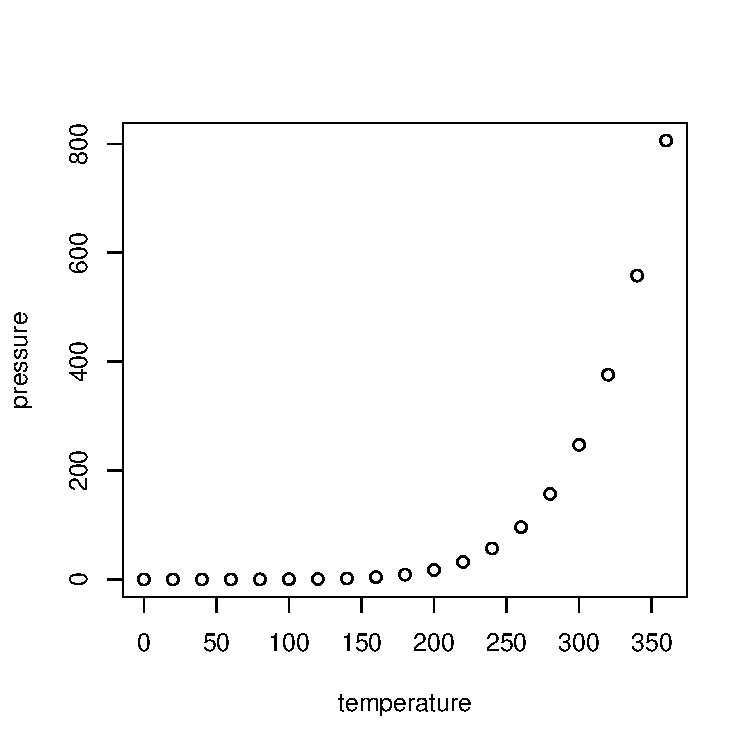
\includegraphics{Monografia_files/figure-latex/pressure-1} \end{center}

Note that the \texttt{echo\ =\ FALSE} parameter was added to the code
chunk to prevent printing of the R code that generated the plot.

\chapter{Referencial Teórico}

\chapter{Metodologia}

\chapter{Resultados}

\chapter{Conclusão}	% No próprio texto é necessário invocar \postextual



\printbibliography

\end{document}
